\documentclass[a4paper,twocolumn]{article}
\usepackage{graphicx}
\usepackage{booktabs}
\usepackage{geometry}
\usepackage{fancyhdr}
\usepackage[skip=2pt]{caption}
\usepackage{indentfirst} 
\usepackage{titling}
\usepackage{float}
\usepackage{svg}

% Adjust the margins to use the full space of A4 paper
\geometry{
  a4paper,
  left=17.018mm,
  right=17.018mm,
  top=20.066mm,
  bottom=12.954mm
}

\DeclareCaptionFormat{custom}
{%
    \scriptsize #1 \scriptsize #3
}
\captionsetup{format=custom}


% Set up the header and footer
\fancypagestyle{plain}{
  \fancyhf{}
  \fancyhead[L]{[FM23201]} % Left header
  \fancyfoot[R]{Supervisor[Prof.Makio Ishihara]} % Center footer
  \renewcommand{\headrulewidth}{0pt} % Remove header line
  \renewcommand{\footrulewidth}{0pt} % Remove footer line
}



\pagestyle{plain}
\setlength{\droptitle}{-4em}     % Eliminate the default vertical space
\addtolength{\droptitle}{-2pt}   % Only a guess. Use this for adjustment
\title{\textbf{\Large Development of a Wearable Haptic Feedback Device for Enhancing Immersion in Virtual Reality}}
\author{\small{Korntawat Witchuvanit (Computer Science and Engineering)}}
\date{\vspace{-3em}}

\begin{document}
\small
\maketitle

% Redefine the section command to use a smaller font size and reduce spacing
\makeatletter
\renewcommand\section{\@startsection{section}{1}{\z@}%
  {-1.0ex \@plus -0.5ex \@minus -.2ex}%  % Adjust the spacing before the section title
  {0.3ex \@plus 0.2ex}%  % Adjust the spacing after the section title
  {\normalfont\normalsize\bfseries}}
\makeatother



\section{Introduction}
Virtual reality (VR) has become a powerful platform that offers immersive experiences across a range of applications, including gaming, training simulations, healthcare, education, and therapy.%\cite{10.3389/frobt.2016.00074}. 
One important aspect of immersion is texture rendering, which is typically achieved through visual and auditory cues. Incorporating haptic feedback for realistic texture perception is a central focus of human-computer interaction (HCI) research, but it still presents challenges. Most existing methods rely on handheld devices, which often restrict natural hand movements.

To overcome these limitations, this research investigates the development and performance of a wearable device equipped with flex sensors, a Motion Processing Unit (MPU), and a coin motor, enabling texture perception at three levels of vibration granularity.

% Virtual reality (VR) provides immersive experiences through multisensory feedback, enhancing user interaction with digital environments. One key aspect of immersion is texture rendering, which is commonly achieved through visual and auditory cues. Incorporating haptic feedback for realistic texture perception is a mainstream of HCI research activities and it still remains a challenge. Most existing methods rely on hand-held devices, often limiting natural hand movements. This research explores the development and performance of a wearable device equipped with flex sensors, a Motion Processing Unit (MPU), and a coin motor, enabling texture perception at three vibration granularities.
% --------------------------------------------------------------
% Virtual reality (VR) has evolved into a powerful platform that provides immersive experiences across various applications, including gaming, training simulations, healthcare, education, and therapy\cite{10.3389/frobt.2016.00074}. By integrating visual, auditory, and interactive elements, VR environments create a strong sense of presence, which significantly enhances user engagement and the perception of realism. One key aspect of immersion is texture rendering, which is commonly achieved through visual and auditory cues. Incorporating haptic feedback for realistic texture perception is a mainstream of HCI research activities, and it still remains a challenge. Most existing methods rely on hand-held devices, often limiting natural hand movements. 
% To address these limitations, this research explores the development and performance of a wearable device equipped with flex sensors, a Motion Processing Unit (MPU), and a coin motor, enabling texture perception at three vibration granularities..

%%%%%%%%%%%%%%%%%%%%%%%%%%%%%%%%%%%%%%%%%%%%%%%%%%%%%%%%%%%%%%
\section{Related Work}
Previous research on haptic feedback in virtual reality (VR) has primarily focused on vibrotactile, force, and thermal methods to enhance tactile realism. Vibrotactile feedback\cite{10.1007/978-3-030-06134-0_25}, known for its compact size, affordability, and rapid response, effectively conveys textures and enhances immersion. A follow-up study\cite{10.1145/3025453.3025812} examines how vibrotactile parameters—such as granularity, amplitude, and timbre—affect texture perception by synchronizing vibrations with user movement. The study finds that granularity influences the perception of bumpiness or smoothness.

In this research, I introduce an innovative pulse-width modulation (PWM) method that modulates vibration cycle rates, rather than using traditional methods like amplitude or frequency control. This approach greatly simplifies hardware requirements, as it requires only one actuator per finger. Despite this simplicity, it still enables precise differentiation of texture properties, such as bumpiness and smoothness.

% Deep-Texture [1] renders shapes and textures of things in VR using a linear resonant actuator and a 1-bar mechanism, employing three frequencies for texture simulation. A follow-up study\cite{10.1145/3025453.3025812} examines how vibrotactile parameters (granularity, amplitude, timbre) affect texture perception by synchronizing vibrations with user movement, finding that granularity influences the perception of bumpiness or smoothness. This research develops a data glove leveraging Pulse Width Modulation (PWM) to modulate granularity for texture rendering and discusses the feasibility of PWM. PWM has the advantage of high tolerance for noise from frequent movement of wires that connect sensors and motors.

%%%%%%%%%%%%%%%%%%%%%%%%%%%%%%%%%%%%%%%%%%%%%%%%%%%%%%%%%%%%%%

\section{Wearable Haptic Feedback Device}
The proposed wearable haptic feedback device (Fig.~\ref{fig:finalglove}) integrates multiple sensors and actuators to enhance natural hand interactions in virtual environments. Flex sensors attached to each finger accurately detect bending and movement, enabling detailed gesture recognition essential for precise virtual interactions, while an MPU-6050 inertial measurement unit (IMU) captures hand orientation, angular velocity, and acceleration data to improve gesture realism during dynamic movements. Core processing is managed by an ESP32 microcontroller, which processes real-time sensor inputs and generates precise pulse-width modulation (PWM) signals to control coin vibration motors at the fingertips. These motors provide realistic vibrotactile sensations, effectively simulating various virtual textures. 

\begin{figure}[H]
  \centering
	\includegraphics[width=0.249\textwidth]{Fig/glove_1.png}%imagine location
	\caption{Finished glove}\label{fig:finalglove}%use name for ref.
\end{figure}


% The proposed device is a sensor-equipped glove designed to enable finger tracking while delivering realistic haptic feedback. The glove integrates multiple key components to enhance interaction and immersion. Flex sensors are attached to each finger, allowing the system to detect bending and movement, accurately measuring the degree of flexion to interpret finger gestures in real time. An MPU is embedded to track hand orientation, acceleration, and rotation, and it enables motion capture and seamless interaction within virtual environments. Micro-vibration motors are placed within the glove to enhance tactile realism and provide haptic feedback, generating subtle vibrations that simulate textures during virtual interactions.

%%%%%%%%%%%%%%%%%%%%%%%%%%%%%%%%%%%%%%%%%%%%%%%%%%%%%%%%%%%%%%
\section{Experimental Setup}
The wearable haptic feedback device developed in this study was linked to the host system. Its onboard microcontroller managed real-time sensor data acquisition and vibration control, while Unity coordinated virtual object interactions and synchronized feedback. The complete setup is shown in Fig.~\ref{fig:experiment}.
\begin{figure}[H]\centering
	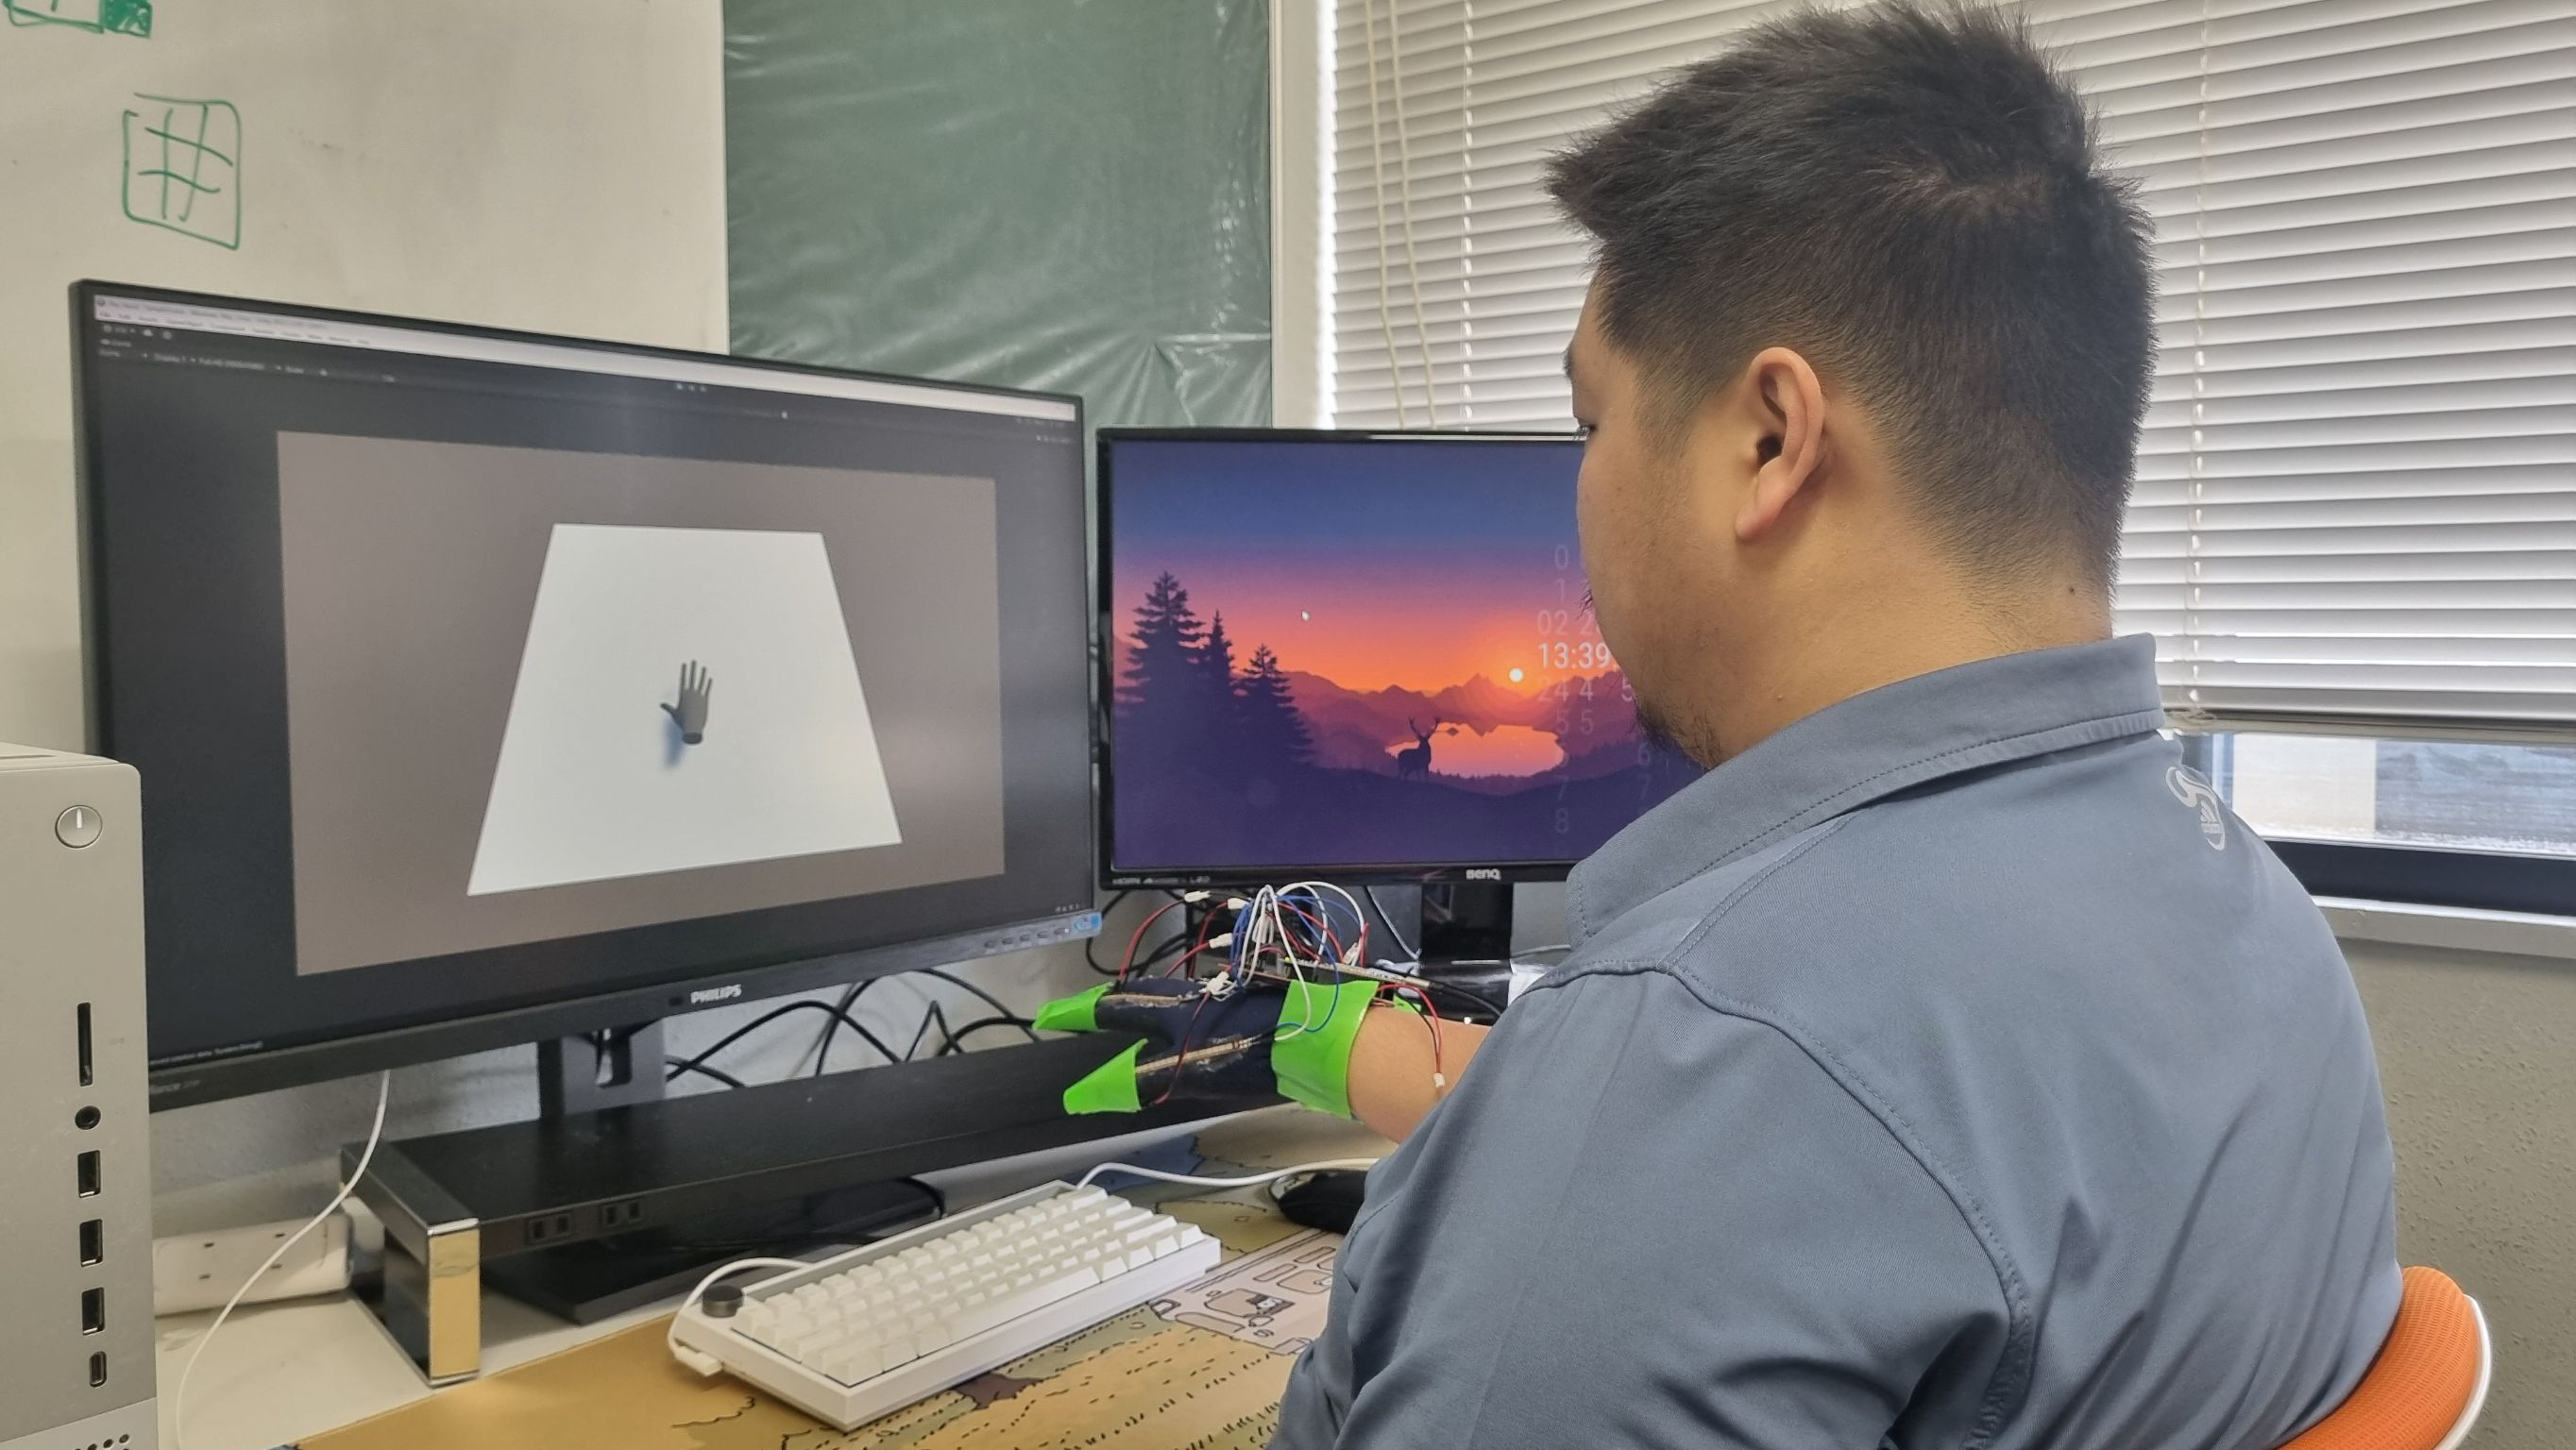
\includegraphics[width=0.3\textwidth]{Fig/experiment.png}%imagine location
	\caption{Overall experimental setup}\label{fig:experiment}%use name for ref.
\end{figure}

Six male participants, aged 24 to 27, took part in a series of experiments to evaluate haptic feedback perception. The haptic feedback was generated using pulse-width modulation (PWM) at three different cycle rates: 0.2, 0.5, and 1.0, with a default frequency of ESP32 at 5000 Hz. Each cycle rate represented a distinct texture sensation.

In the first experiment(Fig.~\ref{fig:ex1}), participants took part in a blind test designed to distinguish between three different types of haptic feedback. Before the test began, they were introduced to all three feedback options. In the virtual environment, a white 3D plane appeared, randomly generating one of the haptic feedback types upon contact with the virtual hand. The participants identified the perceived feedback, repeating the process 15 times(5 times per cycle rate in random order) to assess their ability to differentiate between them.
\begin{figure}[H]\centering
	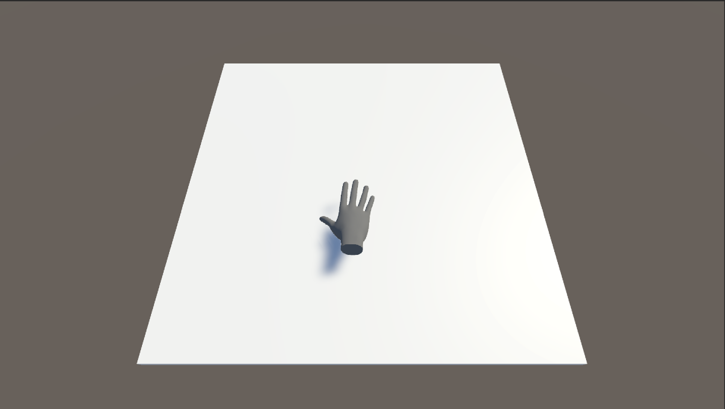
\includegraphics[width=0.3\textwidth]{Fig/ex1.png}%imagine location
	\caption{Experimental setup for Experiment~1}\label{fig:ex1}%use name for ref.
\end{figure}


The result of experiment 1(Fig.~\ref{fig:C_W_ex1}) in identifying vibration cycle rates of 0.2, 0.5, and 1.0 revealed that higher-cycle rate vibrations were more accurately classified. The highest accuracy was at the 1.0 cycle rate, with participants correctly identifying the pattern in 26 out of 30 trials (86.7\%), suggesting that continuous and distinct tactile sensations from shorter pauses enhance perception. Accuracy slightly decreased at the 0.5 cycle rate (80\%) and was lowest at the 0.2 cycle rate (76.7\%), indicating difficulty in distinguishing slower, intermittent tactile sensations. Despite this decline, accuracy remained well above chance (33.3\%), indicating that pulse-width modulation effectively conveys distinct vibrotactile patterns, particularly at higher cycle rates, suitable for realistic virtual texture perception.
\begin{figure}[H]\centering
	\includegraphics[width=0.4\textwidth]{Fig/ex2.png}%imagine location
	\caption{Experimental setup for Experiment~2}\label{fig:ex2}%use name for ref.
\end{figure}

% Six male participants with the ages of 24 to 27 took part in a series of experiment to evaluate haptic feedback perception. The haptic feedback were generated using PWM at three different cycle rates: 0.2, 0.5, and 1.0 with a base frequency of 490Hz, each representing a distinct texture sensation.\par

% In the first experiment, participants conducted a blind test to distinguish between three different haptic feedback. Before starting, they were introduced to all three haptic feedback. A white 3D plane then appeared in the virtual environment, randomly generating one of the feedback upon contact with the virtual hand. The participants identified the perceived feedback, repeating the process 15 times to assess their ability to differentiate between them.\par

% The second experiment explored the relationship between haptic feedback and texture perception. The participants interacted with a textured 3D plane with  three different granularities of brick, grass, or marble, each generating three different haptic feedback. After experiencing all three feedback for a given texture, they were asked to select the one they felt best matched the material before proceeding to the next texture.\par

They completed a total of 12 evaluation questionnaires after the experiments. 			

%%%%%%%%%%%%%%%%%%%%%%%%%%%%%%%%%%%%%%%%%%%%%%%%%%%%%%%%%%%%%%
\section{Results}

The result of experiment 1(Fig.~\ref{fig:C_W_ex1}) in identifying vibration cycle rates of 0.2, 0.5, and 1.0 revealed that higher-cycle rate vibrations were more accurately classified. The highest accuracy was at the 1.0 cycle rate, with participants correctly identifying the pattern in 26 out of 30 trials (86.7\%), suggesting that continuous and distinct tactile sensations from shorter pauses enhance perception. Accuracy slightly decreased at the 0.5 cycle rate (80\%) and was lowest at the 0.2 cycle rate (76.7\%), indicating difficulty in distinguishing slower, intermittent tactile sensations. Despite this decline, accuracy remained well above chance (33.3\%), indicating that pulse-width modulation effectively conveys distinct vibrotactile patterns, particularly at higher cycle rates, suitable for realistic virtual texture perception.

% The results of experiment 1 indicate that in the blind test involving three haptic feedback, the  participants were able to distinguish between the lowest cycle rate (0.2) and the highest one (1.0), as shown in Fig.~\ref{fig:C_W_ex1}. However, the scores for the middle one (0.5) were similar to those of the lowest one. Some participants noted that the glove is too big for my hand, making it difficult to identify the granularities accurately. This may be due to the use of a standard glove with an attached component, which cannot be adjusted to fit every hand.\par

% \begin{figure}[H]\centering
% 	\includesvg[width=0.4\textwidth, inkscapelatex=false]{Fig/ex1_result}
% 	\caption{Participants' accuracy in identifying different vibration cycle rates}\label{fig:ex1_results}
% \end{figure}

\begin{figure}[H]\centering
	\includesvg[width=0.35\textwidth, inkscapelatex=true]{Fig/C_W_Chart}
	\caption{Participants' correct and wrong answers in identifying different vibration cycle rates}\label{fig:C_W_ex1}
\end{figure}

The results of Experiment 2(Fig~\ref{fig:ex2_results}) show that for the brick texture, participants were evenly divided between cycle rates of 0.2 and 0.5. This indicates that both slower and moderate vibrations effectively represented the rough and uneven surface of bricks.
In the case of grass, four participants preferred the medium cycle rate (0.5), while two opted for the slower rate (0.2). This suggests that a moderate rhythmic vibration best matched the semi-rough yet flexible nature of grass.
In contrast, all participants unanimously selected the highest cycle rate (1.0) for the marble texture. This clearly shows that fast, continuous vibration patterns were perceived as most suitable for smooth, polished surfaces like marble.

% The result from the second experiment is shown in Fig.2. The marble which represents the smoothest material is compatible with 1.0 cycle rate while the grass is likely to go with 0.5 cycle rate and the last one that represents the least smoothness is equally for 0.2 and 0.5 cycle rate.

\begin{figure}[H]\centering
	\includesvg[width=0.39\textwidth, inkscapelatex=false]{Fig/ex2_result}
	\caption{Participant-selected cycle rates corresponding to virtual surface textures}\label{fig:ex2_results}
\end{figure}

The statistical analysis of the evaluation questionnaire data (Table~\ref{tab:wilcoxon_category_results}) was conducted across three categories: ``Hand Ownership and Control," ``Realistic and Aligned Tactile Sensations Felt," and ``Immersion." A Wilcoxon Signed-Rank test was used to compare each category’s median score against a neutral baseline of 4.0, the midpoint of the 1–7 Likert scale used in the survey.
In the ``Hand Ownership and Control" category, participants rated their experiences significantly lower than the neutral baseline, with a median score of 3.0 ($p<0.001$). This indicates limited feelings of virtual hand ownership and control, likely influenced by ergonomic issues related to the fit of the gloves.
Conversely, the ``Realistic and Aligned Tactile Sensations Felt" category received significantly higher ratings, with a median score of 5.0 ($p<0.001$). This indicates the successful delivery of realistic tactile sensations to the participants.
The ``Immersion" category showed no significant difference from the neutral baseline, with a median score of 4.0 ($p>0.05$), indicating that the level of immersion was moderate.
Overall, these results highlight the effectiveness of the system in providing tactile realism, while also emphasizing the need for ergonomic improvements to enhance the feeling of embodiment and overall immersion in future prototypes.
\begin{table}[H]
  \small
    \centering
    \caption{Wilcoxon Signed-Rank Test Results for Questionnaire Categories}
    \label{tab:wilcoxon_category_results}
    \begin{tabular}{@{} p{1.5cm} c c c l p{1.5cm} @{}}
        \toprule
        \textbf{Category} & \textbf{N} & \textbf{Median} & \textbf{\textit{p}-value} & \textbf{Sig.} & \textbf{Conclusion} \\
        \midrule
        Hand \\ and Control & 30 & 3.0 & 0.000275 & *** & Sig. lower\\ % Hand Ownership and Control , Significantly lower than Neutral
        \midrule
        Realistic Felt & 30 & 5.0 & 0.000041 & *** & Sig. higher\\ % Realistic and Aligned Tactile Sensations Felt, Significantly higher than Neutral
        \midrule
        Immersion & 12 & 4.0 & 0.102470 & & No sig. diff. \\
        \bottomrule
    \end{tabular}
    \caption*{Note: Significance levels: $^* p < 0.05$, $^{**} p < 0.01$, $^{***} p < 0.001$. The `N' value represents the total count of individual questionnaire responses comprising each category (number of questions in the category $\times$ number of participants).``Hand and Control" refers to the category of "Hand Ownership and Control," while "Realistic Felt" refers to the category of "Realistic and Aligned Tactile Sensations Felt." }
\end{table}

% \begin{figure}[h]
%   \centering
%   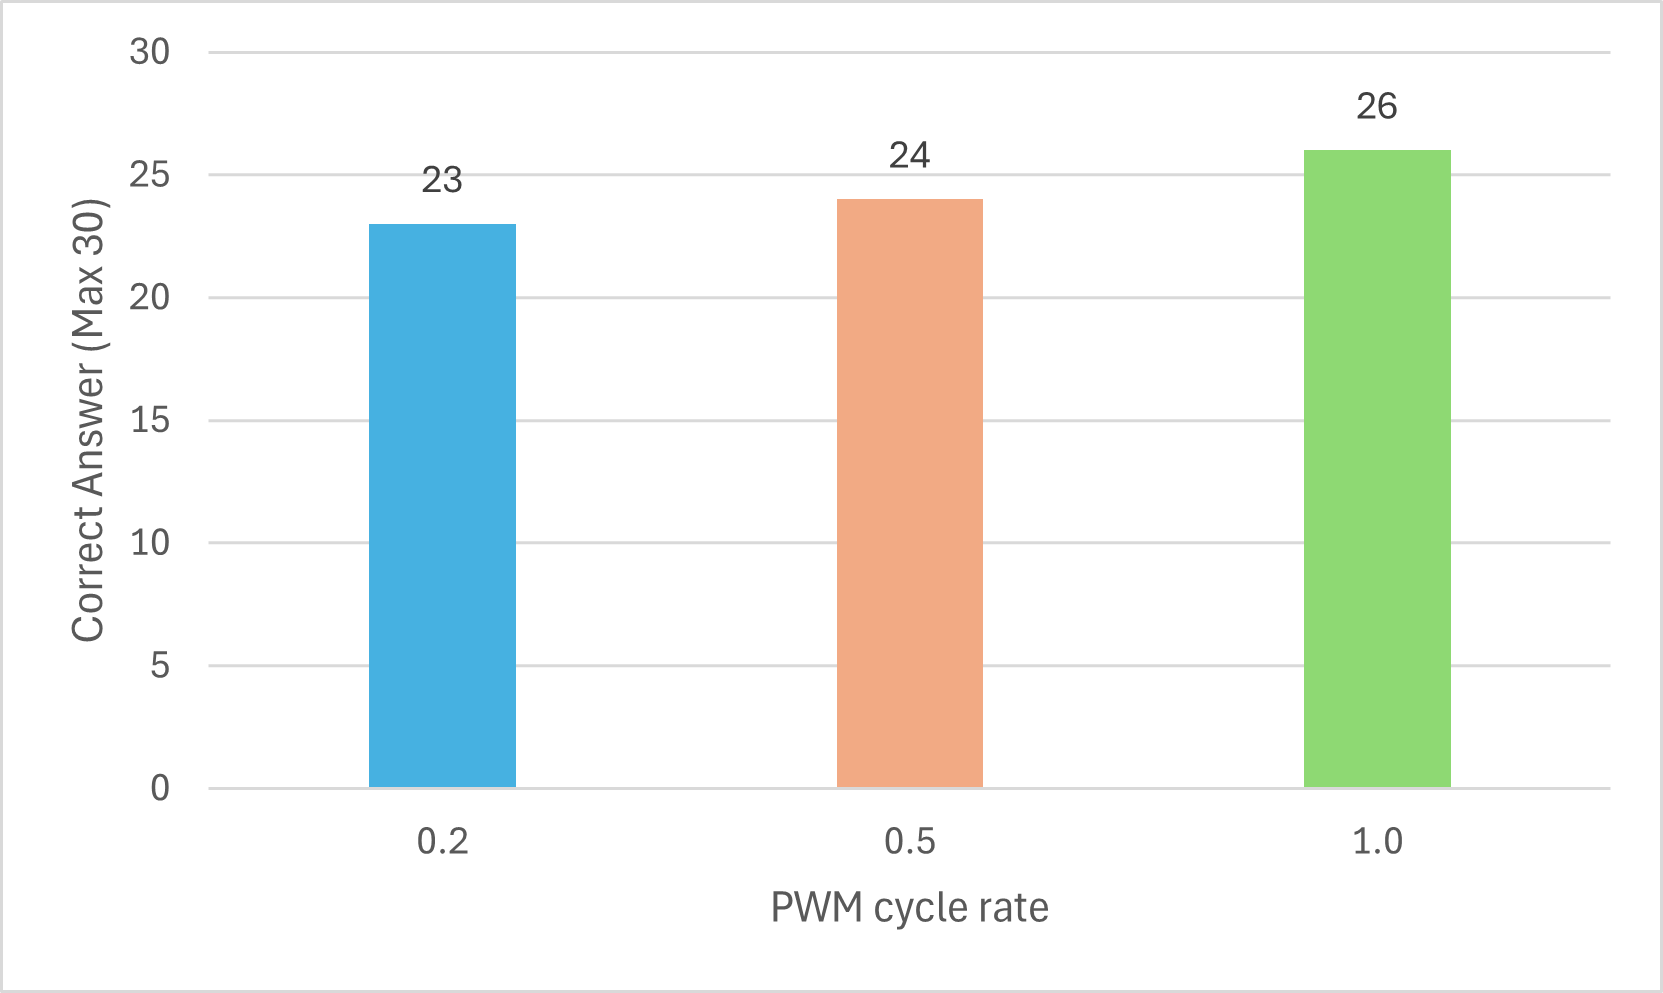
\includegraphics[width=0.35\textwidth]{./Fig/PWM_Correct_Test.png}
%   \caption{{Result of First Experiment}}
%   \label{fig1}
%   \vspace{0.1cm}
%   \centering
%   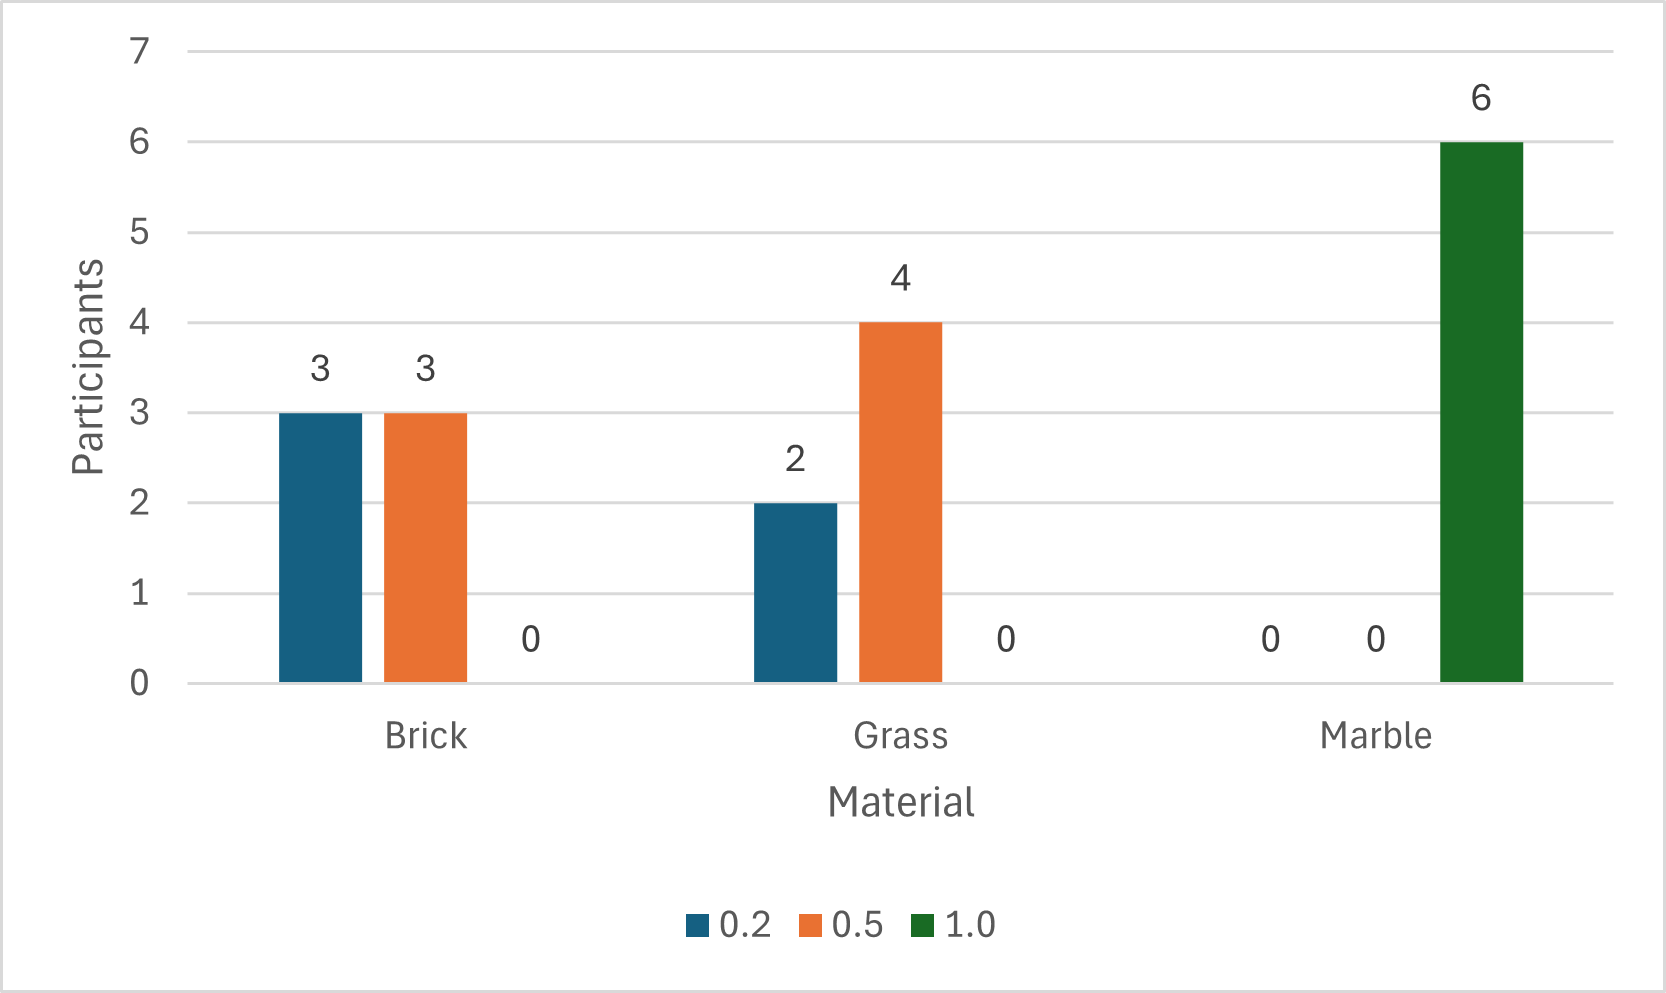
\includegraphics[width=0.35\textwidth]{./Fig/Texture_Select_Test.png}
%   \caption{{Result of Second Experiment}}
%   \label{fig2}
% \end{figure}

%%%%%%%%%%%%%%%%%%%%%%%%%%%%%%%%%%%%%%%%%%%%%%%%%%%%%%%%%%%%%%
\section{Conclusion}
This study aimed to enhance immersion in virtual reality by using a wearable haptic glove equipped with flex sensors, an MPU-6050 IMU, and coin-type vibration motors. The glove employed pulse-width modulation (PWM) to generate tactile feedback. 
Experimental results showed that participants could reliably distinguish between vibration cycle rates that corresponded to textures of varying smoothness, achieving higher accuracy with increased rates. An evaluation questionnaire indicated that the realism of the tactile feedback was significantly higher compared to a neutral baseline.
Future work will focus on optimizing vibration parameters, exploring additional virtual textures, directly comparing PWM-based vibration feedback with other haptic methods, expanding the number of participants for greater statistical robustness, and implementing adaptive feedback algorithms to further enhance immersion and interactivity.
% The results show that participants could distinguish between the lowest cycle rate (0.2) and highest one (1.0) of haptic. Additionally, material smoothness influenced preferred cycle rate, with marble aligning with 1.0 cycle rate, grass with 0.5 cycle rate. These findings highlight the feasibility of PWM for haptic rendering of textures.

%%%%%%%%%%%%%%%%%%%%%%%%%%%%%%%%%%%%%%%%%%%%%%%%%%%%%%%%%%%%%%
\bibliographystyle{ieeetr}
\scriptsize
\bibliography{ref}
\section*{Publication}
  \scriptsize
	\begin{enumerate}
		\bibitem[3]{ieice} K. Witchuvanit and M. Ishihara, “Wearable haptic feedback glove for texture rendering in virtual reality,” in Complex, Intelligent and Software Intensive Systems, Springer Nature Switzerland, 2025, pp. 123–132, isbn: 978-3-031-96099-4.
	\end{enumerate}

\end{document}


% Ref. for Figures and Tables
% \begin{table}[ht]
%     \centering
%     \begin{tabular}{|c|c|c|}
%         \hline
%         Condition & Score & Comment \\
%         \hline
%         A & 5.0 & Good \\
%         B & 3.8 & Average \\
%         C & 2.5 & Poor \\
%         \hline
%     \end{tabular}
%     \caption{Experimental Results}
%     \label{tab:results}
% \end{table}

% \begin{figure}[ht]
%     \centering
%     \includegraphics[width=0.8\linewidth]{example-image} % Replace with your figure
%     \caption{Experimental Result 1}
%     \label{fig:result1}
% \end{figure}